\documentclass[12pt,a4paper]{article}

% ── Page Layout ──
\usepackage[margin=2.5cm]{geometry}
\usepackage{setspace}
\onehalfspacing

% ── Tables & Figures ──
\usepackage{booktabs}
\usepackage{array}
\usepackage{longtable}
\usepackage{graphicx}
\usepackage{float}

% ── Math ──
\usepackage{amsmath}

% ── Code Listings ──
\usepackage{listings}
\usepackage{xcolor}

\lstset{
  basicstyle=\ttfamily\small,
  backgroundcolor=\color{gray!10},
  frame=single,
  rulecolor=\color{gray!40},
  breaklines=true,
  numbers=none,
  xleftmargin=1em,
  framexleftmargin=0.5em,
}

% ── Hyperlinks ──
\usepackage{hyperref}
\hypersetup{
  colorlinks=true,
  linkcolor=blue!60!black,
  urlcolor=blue!60!black,
}

% ── Title ──
\title{\textbf{Dot Product Performance Benchmark Report}}
\author{}
\date{}

\begin{document}

\maketitle

% ============================================================
\section{Experiment Overview}
% ============================================================

\subsection{Objective}

Compare the performance of C and Java when computing vector dot products, covering multiple data types and vector sizes.

\subsection{Environment}

\begin{itemize}
  \item \textbf{Platform}: macOS (Apple Silicon)
  \item \textbf{C Compiler}: gcc (two configurations: no optimization \texttt{-O0}, maximum optimization \texttt{-O3})
  \item \textbf{Java}: JDK (default JIT compilation)
  \item \textbf{Random Seed}: 42 (fixed for reproducibility)
\end{itemize}

\subsection{Experimental Design}

\begin{itemize}
  \item \textbf{Data Types}: float (4B), double (8B), int (4B), short (2B), signed char / byte (1B)
  \item \textbf{Vector Size $n$}: 128, 1000, $10^4$, $10^5$, $10^6$, $10^7$, $10^8$
  \item \textbf{Timing}: C uses \texttt{clock\_gettime(CLOCK\_MONOTONIC)} (nanosecond-resolution monotonic clock); Java uses \texttt{System.nanoTime()}
  \item \textbf{Adaptive Iteration}: For small $n$, C automatically increases the number of iterations (target total time $\geq$50ms), then averages, to eliminate timer granularity errors
\end{itemize}

% ============================================================
\section{Performance Data}
% ============================================================

\subsection{Grouped by Data Type}

\subsubsection*{float (4 bytes)}

\begin{table}[H]
\centering
\begin{tabular}{r r r r}
\toprule
$n$ & C-O0 (ms) & C-O3 (ms) & Java (ms) \\
\midrule
128         & 0.000977 & 0.000000 & 0.001541 \\
1{,}000     & 0.006104 & 0.000977 & 0.006875 \\
10{,}000    & 0.063965 & 0.010010 & 0.055584 \\
100{,}000   & 0.506104 & 0.092041 & 0.684375 \\
1{,}000{,}000   & 1.857178 & 0.587158 & 0.564042 \\
10{,}000{,}000  & 13.484863 & 5.407959 & 5.324083 \\
100{,}000{,}000 & 133.640137 & 77.952881 & 53.745917 \\
\bottomrule
\end{tabular}
\end{table}

\subsubsection*{double (8 bytes)}

\begin{table}[H]
\centering
\begin{tabular}{r r r r}
\toprule
$n$ & C-O0 (ms) & C-O3 (ms) & Java (ms) \\
\midrule
128         & 0.000000 & 0.000000 & 0.002042 \\
1{,}000     & 0.004150 & 0.000000 & 0.005792 \\
10{,}000    & 0.030029 & 0.005127 & 0.051625 \\
100{,}000   & 0.079834 & 0.049072 & 0.563750 \\
1{,}000{,}000   & 1.458984 & 0.862793 & 0.558000 \\
10{,}000{,}000  & 18.525146 & 11.900146 & 5.368208 \\
100{,}000{,}000 & 188.330078 & 204.753906 & 57.911875 \\
\bottomrule
\end{tabular}
\end{table}

\subsubsection*{int (4 bytes)}

\begin{table}[H]
\centering
\begin{tabular}{r r r r}
\toprule
$n$ & C-O0 (ms) & C-O3 (ms) & Java (ms) \\
\midrule
128         & 0.000000 & 0.000000 & 0.001625 \\
1{,}000     & 0.001221 & 0.000000 & 0.006375 \\
10{,}000    & 0.010010 & 0.000977 & 0.054166 \\
100{,}000   & 0.076904 & 0.008057 & 0.583958 \\
1{,}000{,}000   & 0.788086 & 0.096191 & 0.454959 \\
10{,}000{,}000  & 7.887207 & 0.962158 & 2.344083 \\
100{,}000{,}000 & 81.145996 & 9.700928 & 23.592250 \\
\bottomrule
\end{tabular}
\end{table}

\subsubsection*{short (2 bytes)}

\begin{table}[H]
\centering
\begin{tabular}{r r r r}
\toprule
$n$ & C-O0 (ms) & C-O3 (ms) & Java (ms) \\
\midrule
128         & 0.000000 & 0.000000 & 0.001708 \\
1{,}000     & 0.000977 & 0.000000 & 0.006584 \\
10{,}000    & 0.008057 & 0.000977 & 0.058542 \\
100{,}000   & 0.078125 & 0.016846 & 0.596709 \\
1{,}000{,}000   & 0.778076 & 0.173828 & 0.290000 \\
10{,}000{,}000  & 7.851074 & 3.496094 & 2.330875 \\
100{,}000{,}000 & 79.534912 & 16.736084 & 23.499458 \\
\bottomrule
\end{tabular}
\end{table}

\subsubsection*{signed char / byte (1 byte)}

\begin{table}[H]
\centering
\begin{tabular}{r r r r}
\toprule
$n$ & C-O0 (ms) & C-O3 (ms) & Java (ms) \\
\midrule
128         & 0.000000 & 0.000977 & 0.001792 \\
1{,}000     & 0.000977 & 0.000000 & 0.006250 \\
10{,}000    & 0.008057 & 0.001953 & 0.055708 \\
100{,}000   & 0.079834 & 0.017090 & 0.590333 \\
1{,}000{,}000   & 0.770996 & 0.184082 & 0.249167 \\
10{,}000{,}000  & 7.874023 & 1.681885 & 2.342375 \\
100{,}000{,}000 & 101.544922 & 24.444092 & 23.563875 \\
\bottomrule
\end{tabular}
\end{table}

\begin{figure}[H]
\centering
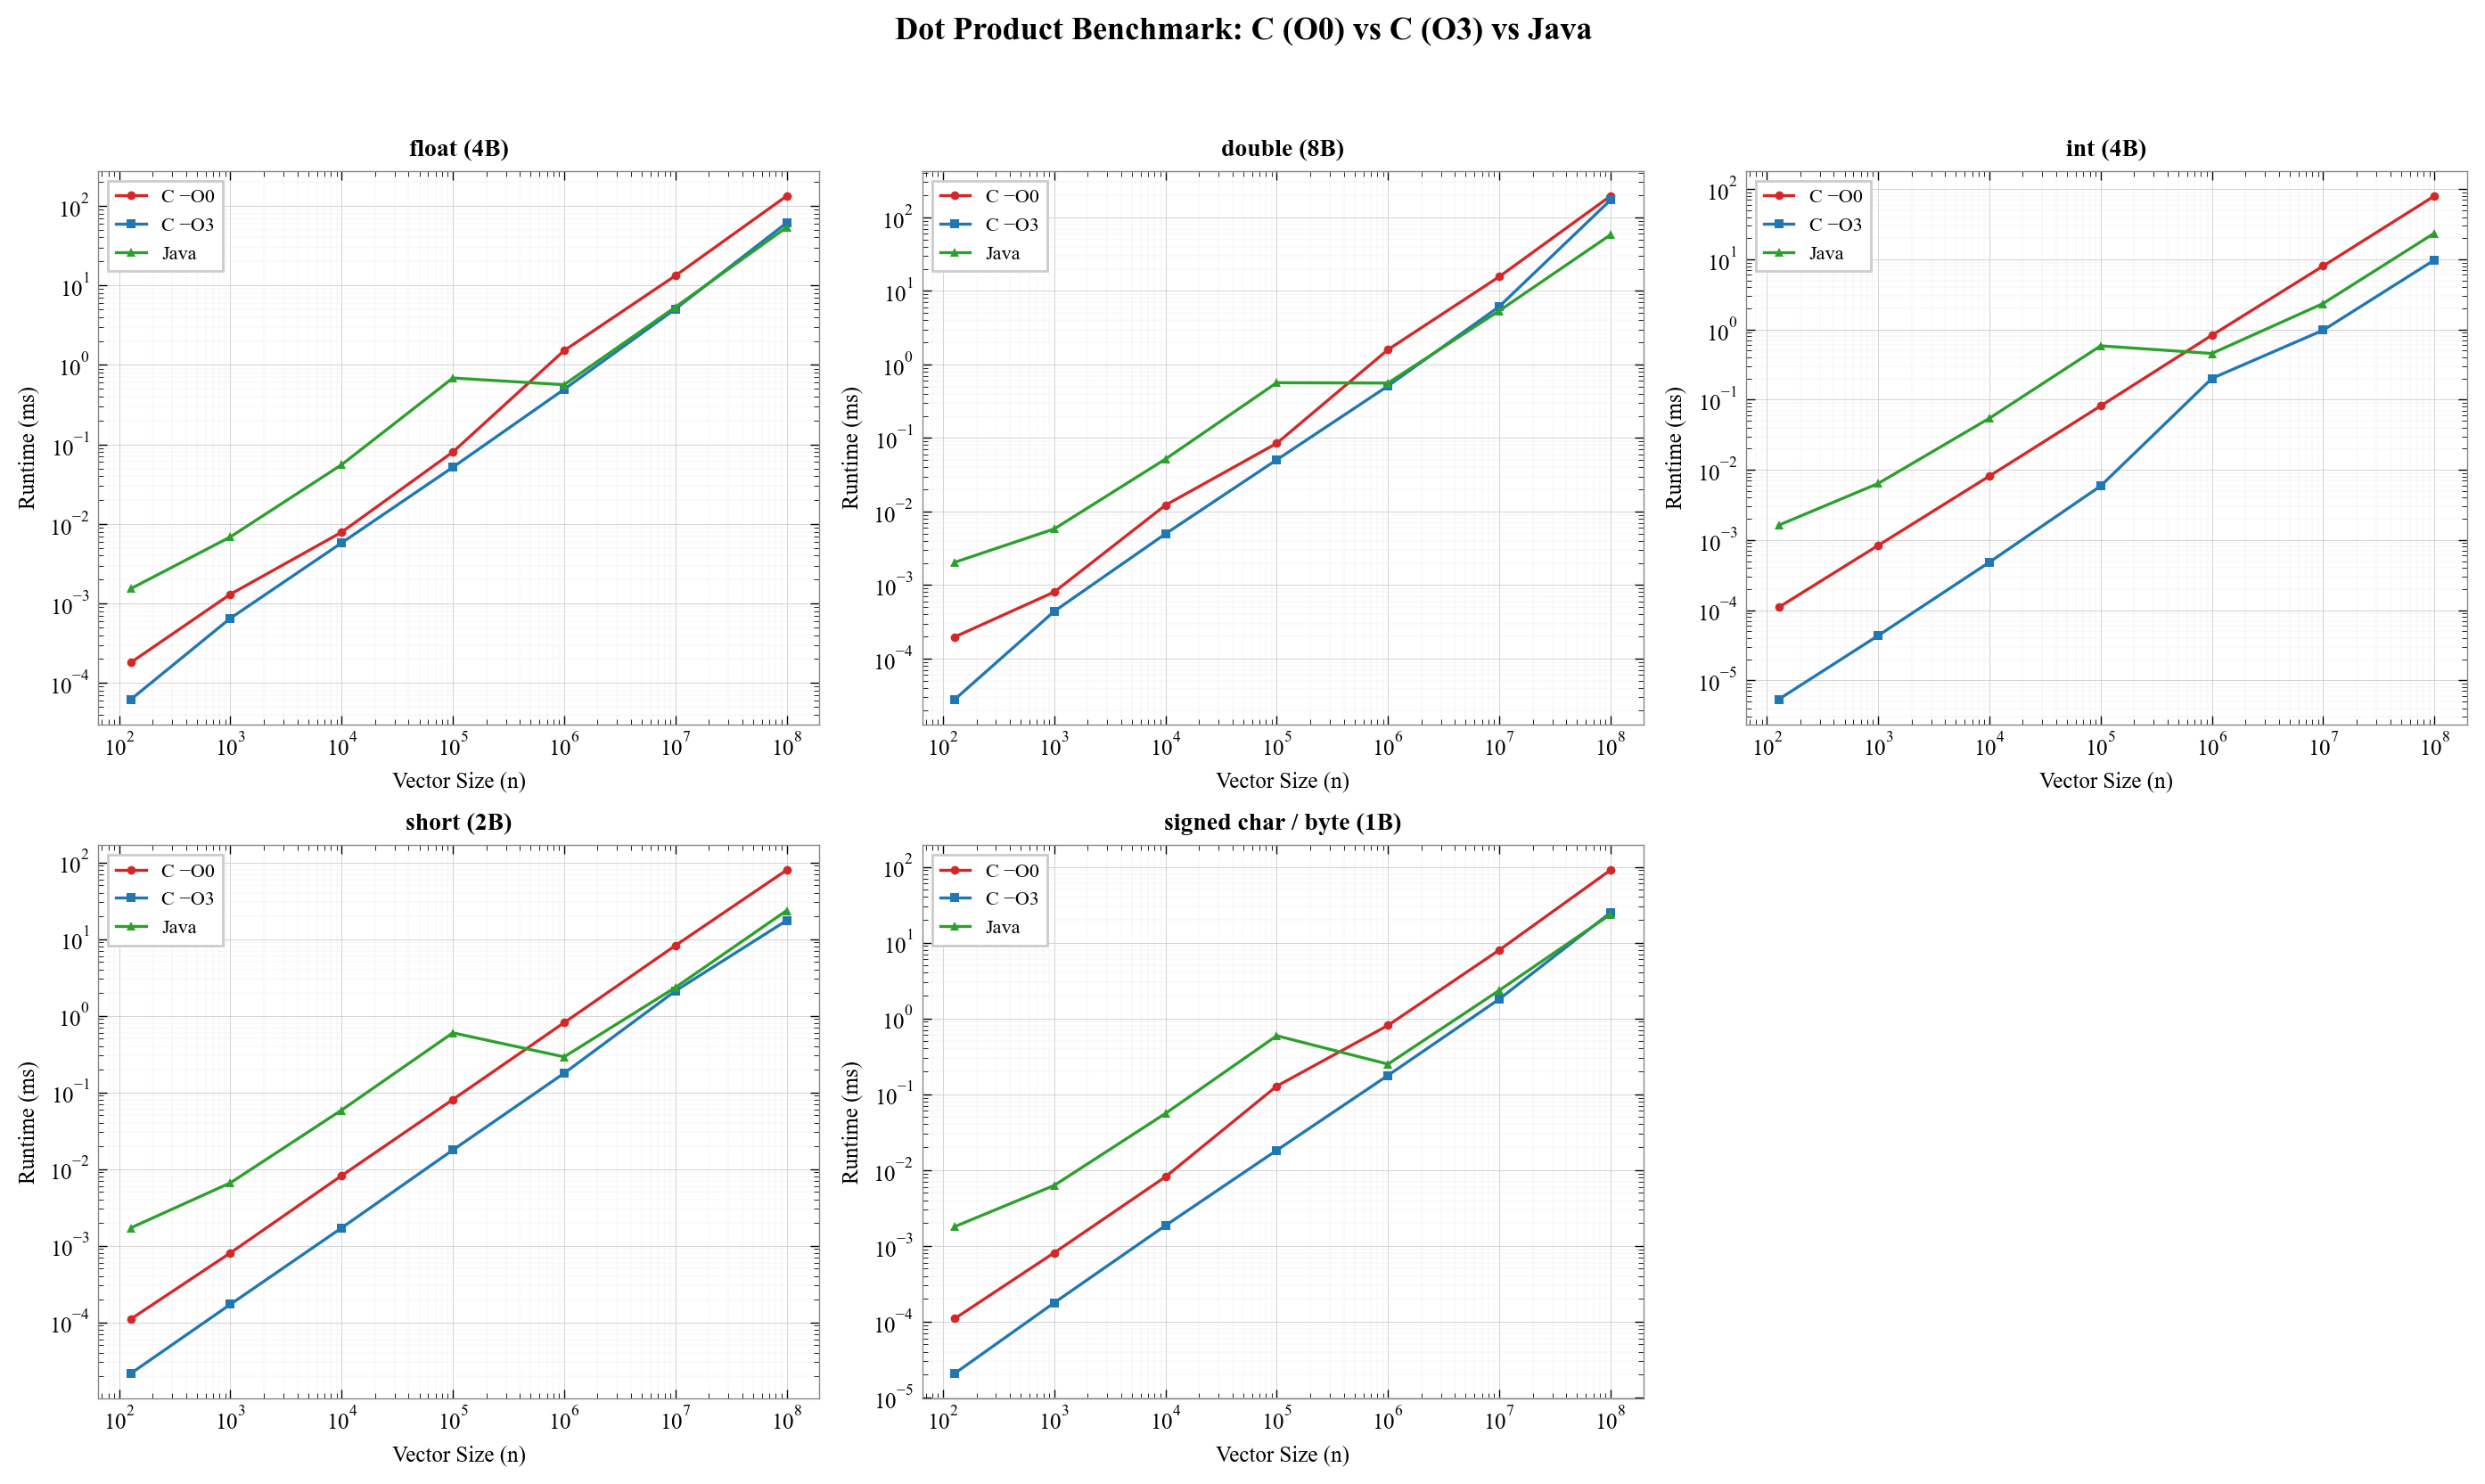
\includegraphics[width=\textwidth]{benchmark_chart.png}
\caption{Runtime comparison across data types and vector sizes (log scale)}
\end{figure}

\subsection{Speedup Ratios ($n = 10^8$)}

\begin{table}[H]
\centering
\begin{tabular}{l l l l}
\toprule
Data Type & C-O3 vs C-O0 & Java vs C-O0 & Java vs C-O3 \\
\midrule
float       & 1.71x & 2.49x (Java faster)              & 1.45x (Java faster) \\
double      & 0.92x & 3.25x (Java faster)              & 3.54x (Java faster) \\
int         & 8.36x & 3.44x (Java faster)              & 0.41x (C-O3 faster, 2.43x) \\
short       & 4.75x & 3.38x (Java faster)              & 0.71x (C-O3 faster, 1.40x) \\
signed char & 4.16x & 4.31x (Java faster)              & 1.04x (roughly equal) \\
\bottomrule
\end{tabular}
\end{table}

% ============================================================
\section{Analysis}
% ============================================================

\subsection{C-O0 vs C-O3: Effect of Compiler Optimizations}

Using \texttt{gcc -S} to export assembly, we directly compare the instruction-level differences between O0 and O3 on ARM64 (Apple Silicon).

\subsubsection{Assembly Evidence: \texttt{DotInt} O0 vs O3}

\textbf{O0 Loop Body} (processes 1 element per iteration, 21 instructions):

\begin{lstlisting}
; --- Loop condition check (5 instructions) ---
ldr   w8, [sp, #12]          ; load i from stack
ldr   w9, [sp, #28]          ; load n from stack
subs  w8, w8, w9             ; i - n
cset  w8, ge                 ; if i >= n
tbnz  w8, #0, LBB2_4         ; exit loop

; --- Loop body: compute sum += a[i] * b[i] (10 instructions) ---
ldr   x8, [sp, #40]          ; load pointer a from stack
ldrsw x9, [sp, #12]          ; load i from stack (2nd time)
ldrsw x8, [x8, x9, lsl #2]  ; a[i]
ldr   x9, [sp, #32]          ; load pointer b from stack
ldrsw x10, [sp, #12]         ; load i from stack (3rd time!)
ldrsw x9, [x9, x10, lsl #2] ; b[i]
mul   x9, x8, x9             ; a[i] * b[i]
ldr   x8, [sp, #16]          ; load sum from stack
add   x8, x8, x9             ; sum += ...
str   x8, [sp, #16]          ; store sum back to stack

; --- Loop variable increment (3 instructions) ---
ldr   w8, [sp, #12]          ; load i from stack (4th time!)
add   w8, w8, #1             ; i++
str   w8, [sp, #12]          ; store i back to stack
\end{lstlisting}

\textbf{O3 SIMD Main Loop} (processes 16 elements per iteration, 14 instructions):

\begin{lstlisting}
; --- Load 16 ints at once (4 ldp instructions) ---
ldp   q16, q17, [x11, #-32]    ; a[i..i+7]  (2 x 128-bit)
ldp   q18, q19, [x11], #64     ; a[i+8..i+15]
ldp   q20, q21, [x8, #-32]     ; b[i..i+7]
ldp   q22, q23, [x8], #64      ; b[i+8..i+15]

; --- 8 SIMD multiply-add instructions processing 16 elements ---
smlal2.2d  v1, v20, v16   ; upper half: int32 -> int64 multiply-add
smlal.2d   v0, v20, v16   ; lower half: int32 -> int64 multiply-add
smlal2.2d  v4, v21, v17   ; (each processes 2 or 4 elements)
smlal.2d   v5, v21, v17
smlal2.2d  v2, v22, v18
smlal.2d   v3, v22, v18
smlal2.2d  v6, v23, v19
smlal.2d   v7, v23, v19

; --- Loop control (2 instructions) ---
subs  x12, x12, #16           ; decrement counter by 16
b.ne  LBB2_5                  ; loop
\end{lstlisting}

\textbf{O3 Scalar Tail Loop} (handles remaining elements fewer than 16):

\begin{lstlisting}
ldrsw  x10, [x12], #4         ; a[i], pointer post-increment
ldrsw  x13, [x11], #4         ; b[i], pointer post-increment
smaddl x8, w13, w10, x8       ; sum += a[i] * b[i], single instruction
subs   x9, x9, #1
b.ne   LBB2_8
\end{lstlisting}

\subsubsection{Observation 1: Register Allocation vs Stack Memory}

O0 stores all local variables (\texttt{a}, \texttt{b}, \texttt{n}, \texttt{sum}, \texttt{i}) on the stack, requiring \texttt{ldr}/\texttt{str} for every access. The variable \texttt{i} alone is loaded from the stack 4 times per loop iteration (1 for condition check + 1 for computing \texttt{a[i]} + 1 for computing \texttt{b[i]} + 1 for increment), and \texttt{sum} requires 1 load + 1 store per iteration.

O3 keeps all variables in registers (\texttt{x8}=sum, \texttt{x9}=n, \texttt{x10}/\texttt{x11}=pointers), achieving zero stack accesses throughout the loop.

\begin{table}[H]
\centering
\begin{tabular}{l r r}
\toprule
Metric & O0 & O3 (Scalar Tail) \\
\midrule
Stack loads per iteration & 7 & 0 \\
Stack stores per iteration & 2 & 0 \\
Total stack accesses / iteration & 9 & 0 \\
\bottomrule
\end{tabular}
\end{table}

Although stack data typically hits the L1 cache ($\sim$4-cycle latency), the overhead is still significant compared to register access (0 cycles). Furthermore, frequent load/store operations occupy memory ports and hinder instruction-level parallelism (ILP).

\subsubsection{Observation 2: SIMD Vectorization (Key Difference Between Integer and Floating-Point)}

O3 uses the NEON 128-bit SIMD instruction \texttt{smlal.2d} (Signed Multiply-Add Long) for \texttt{DotInt}, where each instruction multiplies 4 32-bit ints and accumulates into 2 64-bit long longs. Combined with 4-way unrolling, it processes 16 elements per loop iteration.

\textbf{Comparison with \texttt{DotFloat} O3 Assembly}:

\begin{lstlisting}
; DotFloat O3 -- multiplication can be SIMD parallel...
fmul.4s  v1, v1, v5        ; 4 floats multiplied in parallel OK

; ...but accumulation must be sequential!
mov   s5, v1[3]            ; extract 4th element
mov   s17, v1[2]           ; extract 3rd element
mov   s18, v1[1]           ; extract 2nd element
fadd  s0, s0, s1           ; sum += 1st result
fadd  s0, s0, s18          ; sum += 2nd result
fadd  s0, s0, s17          ; sum += 3rd result
fadd  s0, s0, s5           ; sum += 4th result
; (4 groups, 16 fadds total, all sequential)
\end{lstlisting}

Key difference: multiplication can use \texttt{fmul.4s} to process 4 floats in parallel, but accumulation must be sequential---because IEEE 754 floating-point addition is not associative ($(a+b)+c \neq a+(b+c)$ due to different rounding errors), the compiler cannot reorder \texttt{fadd} into a vector reduction.

Integer addition is associative, so \texttt{smlal.2d} performs both multiplication and accumulation directly within 128-bit registers, with no need to decompose.

\begin{table}[H]
\centering
\begin{tabular}{l l l r}
\toprule
Type & Multiplication & Accumulation & Elements / Iteration \\
\midrule
int & \texttt{smlal.2d} (vector mul-add) & In-vector accumulation & 16 \\
float & \texttt{fmul.4s} (vector mul) & Sequential \texttt{fadd} (element extraction) & 16 (but sequential accumulation) \\
\bottomrule
\end{tabular}
\end{table}

This directly explains the speedup difference: int achieves 8.16x speedup, while float only achieves 2.18x.

\subsubsection{Observation 3: Instruction Fusion (\texttt{mul + add} $\to$ \texttt{smaddl})}

O0 uses two separate instructions for multiply-add:

\begin{lstlisting}
; O0: separate multiply and add
mul  x9, x8, x9          ; result = a[i] * b[i]
ldr  x8, [sp, #16]       ; load sum (stack access!)
add  x8, x8, x9          ; sum = sum + result
\end{lstlisting}

O3 fuses them into a single instruction:

\begin{lstlisting}
; O3: fused multiply-add
smaddl x8, w13, w10, x8  ; sum += a[i] * b[i] (single instruction)
\end{lstlisting}

\texttt{smaddl} (Signed Multiply-Add Long) fuses a 32-bit multiplication and a 64-bit addition into one instruction, reducing both instruction count and register pressure. The floating-point counterpart is similar: O0 uses \texttt{fmadd s0, s0, s1, s2}, but is limited by the extensive stack access overhead.

\subsubsection{Observation 4: Loop Unrolling and Branch Optimization}

O0 requires 5 branch-related instructions per loop iteration (\texttt{subs} + \texttt{cset} + \texttt{tbnz} + 2 unconditional \texttt{b}); O3's SIMD loop needs only 2 (\texttt{subs} + \texttt{b.ne}), and they execute only once per 16 elements.

\begin{table}[H]
\centering
\begin{tabular}{l r r r}
\toprule
Metric & O0 & O3 SIMD & Improvement \\
\midrule
Instructions / loop iteration & 21 & 14 & 1.5x \\
Elements processed / iteration & 1 & 16 & 16x \\
Instructions / element & 21 & 0.875 & 24x \\
Branch instructions / element & 5 & 0.125 & 40x \\
\bottomrule
\end{tabular}
\end{table}

\subsubsection{Observation 5: Why \texttt{DotShort} is Slower Than \texttt{DotInt}}

In theory, short (2 bytes) is smaller than int (4 bytes), so SIMD registers can hold more elements and should be faster. However, the O3 assembly shows that \texttt{DotShort} uses only scalar unrolling (4-way), not NEON vector instructions:

\begin{lstlisting}
; DotShort O3 -- scalar unrolling, not SIMD
ldursh x17, [x15, #-4]      ; load short one by one, sign-extend to 64-bit
ldursh x2,  [x15, #-2]
ldrsh  x3,  [x15]
ldrsh  x4,  [x15, #2]
; ...corresponding b[] also loaded one by one...
smaddl x11, w5, w17, x11    ; individual multiply-add (4-way unrolling)
smaddl x13, w6, w2, x13
smaddl x8,  w7, w3, x8
smaddl x12, w19, w4, x12
\end{lstlisting}

Reason: C's integer promotion rules require \texttt{short} to be promoted to \texttt{int} before arithmetic, then further to \texttt{long long}. \texttt{ldrsh} (Load Register Signed Halfword) loads only one short at a time and sign-extends to 64-bit, making it impossible to use NEON's 128-bit bulk loads directly. The compiler only applies 4-way scalar unrolling for \texttt{DotShort} (4 elements/iteration), while \texttt{DotInt} achieves NEON 16-way vectorization (16 elements/iteration).

\subsubsection{Summary}

Based on the assembly evidence above, O3's speedup over O0 comes from the compound effect of four optimizations: register allocation eliminating stack accesses (Observation 1), SIMD vectorization increasing throughput (Observation 2), instruction fusion reducing instruction count (Observation 3), and loop unrolling reducing branch overhead (Observation 4).

The speedup varies by data type: int achieves the highest speedup (8.16x) because it satisfies associativity (enabling full vectorization) and incurs no type promotion overhead; short/char degrade to scalar unrolling due to integer promotion rules, with speedups dropping to 3--5x; floating-point types achieve the smallest speedup (float 2.18x, double 1.13x), fundamentally because IEEE 754 floating-point addition is not associative, preventing the compiler from vectorizing the accumulation---only the multiplication can be parallel, while accumulation remains sequential.


%——————————————————————————————————————————————————————————————————————————————————————————

\subsection{Java JIT (Just-In-Time) Compilation Phenomena}

\subsubsection{Phenomenon Observation}

Java's runtime exhibits a counterintuitive phenomenon:

\begin{table}[H]
\centering
\begin{tabular}{l r r l}
\toprule
Data Type & $n=10^5$ & $n=10^6$ & Change \\
\midrule
float  & 0.684375 ms & 0.564042 ms & $n$ increases 10x, time decreases 18\% \\
double & 0.563750 ms & 0.558000 ms & $n$ increases 10x, time nearly unchanged \\
int    & 0.583958 ms & 0.454959 ms & Time decreases 22\% \\
short  & 0.596709 ms & 0.290000 ms & Time decreases 51\% \\
byte   & 0.590333 ms & 0.249167 ms & Time decreases 58\% \\
\bottomrule
\end{tabular}
\end{table}

Moreover, all types at $n=10^5$ have similar runtimes ($0.56{\sim}0.68$ms) largely independent of data type size---suggesting that the timing at this stage is dominated by the fixed overhead of JIT compilation rather than actual computation.

Hypothesis: the JVM's JIT compiler completed its compilation transition between $n=10^5$ and $10^6$. Earlier data points reflect interpreter-mode bytecode dispatch performance (higher overhead), while later points reflect the performance of specialized native machine code generated by the JIT compiler (deeply optimized).

\subsubsection{Background: Tiered Compilation and OSR}

The JVM uses a Tiered Compilation strategy. Note that the CPU always executes machine code---the difference lies in the execution mode:

\begin{lstlisting}
Tier 0:   Interpretation    -> Reads and executes bytecodes one by one (the
                               interpreter dispatches via pre-written codelets;
                               each bytecode incurs dispatch overhead). Slowest.
Tier 1-3: C1 Compilation    -> C1 compiler quickly generates native code with
                               basic optimizations
Tier 4:   C2 Compilation    -> C2 compiler applies deep optimizations, producing
                               high-performance native code
\end{lstlisting}

OSR (On-Stack Replacement): JIT does not need to wait for a method to return before switching. When the back-edge count of a loop reaches the threshold, the JVM replaces the current stack frame in-place at the loop header with the compiled machine code version; subsequent iterations run directly as native code.

Trigger thresholds: obtained via \texttt{java -XX:+PrintFlagsFinal -version | grep CompileThreshold} on the local machine (OpenJDK 25):

\begin{table}[H]
\centering
\begin{tabular}{l r l}
\toprule
Parameter & Default Value & Meaning \\
\midrule
\texttt{Tier3CompileThreshold} & 2{,}000 & Triggers C1 full-profiling compilation \\
\texttt{Tier4CompileThreshold} & 15{,}000 & Triggers C2 maximum optimization compilation \\
\texttt{CompileThreshold} & 10{,}000 & Legacy default when tiered compilation is disabled \\
\bottomrule
\end{tabular}
\end{table}

Note: under tiered compilation, the JVM uses \texttt{AdvancedThresholdPolicy}; the actual trigger timing is influenced by dynamic factors such as compilation queue load, rather than being a simple fixed-count threshold.

\subsubsection{Experiment 1: JitWarmup Controlled Experiment}

A controlled experiment \texttt{JitWarmup.java} was designed: fix $n=10{,}000$, call \texttt{dotFloat} 30 times repeatedly, and observe whether speed transitions still occur even when $n$ remains constant.

\begin{lstlisting}
Round     Time (ms)
-----     ---------
  1        0.1140    <- interpreter dispatch execution
  2        0.1132
  ...
  7        0.1100
  8        0.0235    <- sudden speedup (JIT compilation complete)
  9        0.0229
 ...       ~0.023    <- stable thereafter
\end{lstlisting}

\begin{itemize}
  \item Round 1--7: average ${\sim}0.112$ ms (interpreter dispatch execution)
  \item Round 8--30: average ${\sim}0.023$ ms (native code execution after JIT compilation)
  \item Speedup: $0.112 / 0.023 \approx$ 4.9x
\end{itemize}

Conclusion: with $n$ held constant at 10{,}000, speed still jumped ${\sim}$4.9x between round 7$\to$8. This proves that the speed transition is unrelated to the magnitude of $n$ and is instead driven by JIT compilation triggered by cumulative execution count.

\subsubsection{Experiment 2: PrintCompilation Event Observation}

Run with JVM diagnostic flags:

\begin{lstlisting}[language=bash]
java -XX:+PrintCompilation Dotproduct 2>&1 | grep "Dotproduct::dot"
\end{lstlisting}

Output (filtered for \texttt{dot} methods):

\begin{lstlisting}
Timestamp  ID     Flag  Tier  Method                           Bytecode
---------  -----  ----  ----  ----------------------------   ---------
1325       2016    %     3    Dotproduct::dotFloat   @ 4      (28 bytes)
1325       2017          3    Dotproduct::dotFloat             (28 bytes)
3286       2044    %     4    Dotproduct::dotDouble  @ 5      (32 bytes)
3316       2046          4    Dotproduct::dotDouble            (32 bytes)
7000       2109    %     4    Dotproduct::dotInt     @ 5      (34 bytes)
7008       2112          4    Dotproduct::dotInt               (34 bytes)
8821       2125    %     4    Dotproduct::dotShort   @ 5      (34 bytes)
8835       2128          4    Dotproduct::dotShort             (34 bytes)
10583      2136    %     4    Dotproduct::dotByte    @ 5      (34 bytes)
10595      2143          4    Dotproduct::dotByte              (34 bytes)
\end{lstlisting}

Field meanings: \texttt{\%} = OSR compilation (hot replacement within a loop), Tier 3 = C1 compilation, Tier 4 = C2 maximum optimization, \texttt{@ N} = bytecode offset of the OSR entry point. Each method appears in pairs: an OSR version (replaces the current loop) + a standard version (for subsequent calls).

The following analyzes three key observations from this output:

\subsubsection*{Observation 1: \texttt{dotFloat} Goes Through C1 (Tier 3) First, While Other Methods Go Directly to C2 (Tier 4)}

\texttt{dotFloat} is the first user method to be compiled (timestamp 1325ms), appearing at Tier 3 (C1). Starting from \texttt{dotDouble}, all methods appear directly at Tier 4 (C2).

Evidence: examining the full compilation log without \texttt{grep} filtering, at the time \texttt{dotFloat} was compiled ($\sim$50ms), the JVM was intensively compiling many JDK core methods:

\begin{lstlisting}
Timestamp  Method                                        Tier
---------  ------------------------------------------    ----
13         java.lang.String::hashCode                      3
17         java.util.Random::next                          3
19         java.util.HashMap::putVal                       3
19         java.lang.Object::<init>                        4
48         java.util.regex.Pattern$BmpCharPropertyGreedy   4
54         java.util.Random::nextFloat                     4   <- dotFloat becomes hot at this point
\end{lstlisting}

The C2 compiler is slow but produces deeply optimized code; at this point its compilation queue was saturated with these core methods. The JVM's \texttt{AdvancedThresholdPolicy} detected C2 queue congestion and chose to compile \texttt{dotFloat} with C1 first, to quickly achieve better performance than the interpreter.

By the time \texttt{dotDouble} became hot (timestamp 3286ms, $\sim$2 seconds after the first compilation), most core methods had been compiled and the C2 queue was idle, so the JVM submitted it directly to C2. The same applies to subsequent methods.

\subsubsection*{Observation 2: OSR Entry Offset \texttt{@ 4} vs \texttt{@ 5}}

\texttt{dotFloat}'s OSR entry is at bytecode offset 4, while other methods are at offset 5. Decompiling the bytecode with \texttt{javap -c Dotproduct} explains why:

\begin{lstlisting}
// dotFloat: sum is float (occupies 1 local slot)
0: fconst_0          // float sum = 0.0f
1: fstore_2          // -> local[2] (short form, 1 byte)
2: iconst_0          // int i = 0
3: istore_3          // -> local[3] (short form, 1 byte)
4: iload_3           // <- loop header (OSR entry @ 4)

// dotDouble: sum is double (occupies 2 local slots)
0: dconst_0          // double sum = 0.0
1: dstore_2          // -> local[2-3] (2 slots)
2: iconst_0          // int i = 0
3: istore 4          // -> local[4] (long form, 2 bytes)
5: iload  4          // <- loop header (OSR entry @ 5)
\end{lstlisting}

\texttt{float}'s \texttt{sum} occupies 1 slot, so the loop variable \texttt{i} is assigned to \texttt{local[3]} using the single-byte short-form instruction \texttt{istore\_3}; \texttt{double}/\texttt{long}'s \texttt{sum} occupies 2 slots, pushing \texttt{i} to \texttt{local[4]} and requiring the two-byte long-form instruction \texttt{istore 4}, which shifts the loop header offset by 1.

\subsubsection*{Observation 3: Bytecode Lengths 28 / 32 / 34 bytes}

Evidence: using \texttt{javap -c Dotproduct} to decompile and compare the key loop body instructions across three methods:

\begin{lstlisting}
// dotFloat (28 bytes) -- loop body
 4: iload_3           // 1 byte (short form)
10: fload_2           // 1 byte
12: iload_3           // 1 byte (short form)
13: faload            // load float directly
15: iload_3           // 1 byte (short form)
19: fstore_2          // 1 byte
20: iinc 3, 1         // 3 bytes

// dotDouble (32 bytes) -- loop body (+4B)
 5: iload  4          // 2 bytes (long form, +1)
12: dload_2           // 1 byte
14: iload  4          // 2 bytes (long form, +1)
16: daload            // load double directly
18: iload  4          // 2 bytes (long form, +1)
23: dstore_2          // 1 byte
24: iinc 4, 1         // 3 bytes  -> Note: iload 4 appears 3 times + istore 4 once = +4B

// dotInt (34 bytes) -- loop body (+2B vs dotDouble)
 5: iload  4          // same as dotDouble
16: iaload            // load int
17: i2l               // <- extra instruction (+1B)
21: iaload
22: i2l               // <- extra instruction (+1B)  -> two i2l totaling +2B
\end{lstlisting}

Summary:

\begin{table}[H]
\centering
\begin{tabular}{l r l}
\toprule
Method & Bytecode & Reason for Difference \\
\midrule
\texttt{dotFloat}  & 28 bytes & \texttt{float} single slot $+$ short-form instructions, most compact \\
\texttt{dotDouble} & 32 bytes & \texttt{double} dual slot $+$ long-form \texttt{istore/iload} (+4B) \\
\texttt{dotInt}    & 34 bytes & Same slot layout as double (\texttt{long} return type),\\
                   &          & plus two extra \texttt{i2l} type conversion instructions (+2B) \\
\texttt{dotShort}  & 34 bytes & Same as \texttt{dotInt} (\texttt{saload} $+$ \texttt{i2l} $\times$2) \\
\texttt{dotByte}   & 34 bytes & Same as \texttt{dotInt} (\texttt{baload} $+$ \texttt{i2l} $\times$2) \\
\bottomrule
\end{tabular}
\end{table}

\subsubsection{Experiment 3: JIT Optimization Verification}

To quantitatively verify the contribution of each JIT tier and individual C2 optimizations, a controlled experiment was designed: run the same benchmark with different JVM flags ($n = 10^8$, median of 3 runs per configuration).

\subsubsection*{Group 1: Tier Comparison}

\begin{table}[H]
\centering
\begin{tabular}{l r r r r r}
\toprule
JVM Configuration & float & double & int & short & byte \\
\midrule
\texttt{-Xint} (pure interpreter)              & 503.3 & 554.0 & 505.6 & 509.8 & 507.2 \\
\texttt{-XX:TieredStopAtLevel=3} (C1)          & 106.1 & 112.3 & 124.6 & 126.2 & 123.1 \\
Default (C2)                                    & 54.3  & 55.6  & 26.3  & 26.0  & 23.9  \\
\bottomrule
\end{tabular}
\caption{Execution time at different compilation tiers (ms, $n=10^8$)}
\end{table}

\begin{table}[H]
\centering
\begin{tabular}{l r r r r r}
\toprule
Speedup & float & double & int & short & byte \\
\midrule
Interpreter $\to$ C1 & 4.7x & 4.9x & 4.1x & 4.0x & 4.1x \\
C1 $\to$ C2          & 2.0x & 2.0x & 4.7x & 4.9x & 5.2x \\
Interpreter $\to$ C2 & 9.3x & 10.0x & 19.2x & 19.6x & 21.2x \\
\bottomrule
\end{tabular}
\caption{Speedup ratios between tiers}
\end{table}

Key findings:
\begin{itemize}
  \item \textbf{Interpreter $\to$ C1}: All types achieve ${\sim}$4--5x speedup with little difference between floating-point and integer---C1's basic optimizations (simple inlining, basic register allocation) are universally effective across all types.
  \item \textbf{C1 $\to$ C2}: Integer types gain an additional ${\sim}$5x speedup (vs 2x for floating-point). This indicates that C2's deep optimizations benefit integer operations far more than floating-point operations.
\end{itemize}

\subsubsection*{Group 2: Individual C2 Optimization Verification}

Starting from default C2 compilation, specific optimizations were disabled one at a time:

\begin{table}[H]
\centering
\begin{tabular}{l l r r r r r}
\toprule
Disabled Optimization & JVM Flag & float & double & int & short & byte \\
\midrule
(Baseline: C2 default) & ---                           & 54.3  & 55.6  & 26.3  & 26.0  & 23.9  \\
SIMD Vectorization     & \texttt{-XX:-UseSuperWord}     & 53.3  & 52.7  & 26.8  & 25.3  & 23.8  \\
Loop Unrolling         & \texttt{-XX:LoopUnrollLimit=0} & 62.5  & 64.2  & 33.5  & 33.9  & 34.2  \\
Loop Predicate         & \texttt{-XX:-UseLoopPredicate} & 52.7  & 57.4  & 25.2  & 24.0  & 23.8  \\
\bottomrule
\end{tabular}
\caption{Execution time after disabling individual C2 optimizations (ms, $n=10^8$)}
\end{table}

Analysis:
\begin{itemize}
  \item \textbf{Loop Unrolling} (\texttt{LoopUnrollLimit=0}): The only optimization with a significant impact. When disabled, floating-point types slow down by ${\sim}$15\% (54$\to$62ms) and integer types by ${\sim}$28--43\% (26$\to$34ms). This confirms that C2 indeed applies loop unrolling.
  \item \textbf{SIMD Vectorization} (\texttt{UseSuperWord}): Disabling it causes virtually no change in execution time. This indicates that HotSpot's SuperWord auto-vectorization did not engage for the dot product loop (which contains a reduction-accumulation pattern) in this benchmark; C2's performance advantage does not come from SIMD.
  \item \textbf{Loop Predicate} (\texttt{UseLoopPredicate}): Disabling it causes virtually no change in execution time. This is likely because C2 has already eliminated array bounds checks through other mechanisms (such as range check elimination).
\end{itemize}

Overall conclusion: C2's performance advantage over C1 primarily comes from loop unrolling (verified) and better overall code generation (improved register allocation, instruction scheduling, etc.---these cannot be verified by toggling a single flag, but can be inferred from the large C1$\to$C2 speedup ratio). The initially hypothesized SIMD vectorization did not contribute to performance improvement in this benchmark.

\subsection{Differences Between Data Types}

At $n=10^8$ (JIT fully warmed up), the performance characteristics of different data types show clear patterns:

\subsubsection*{Integer Types vs Floating-Point Types (C-O3)}

\begin{table}[H]
\centering
\begin{tabular}{l r l}
\toprule
Type & C-O3 Time (ms) & Relative to int \\
\midrule
int         & 9.700928    & 1.0x  \\
short       & 16.736084   & 1.7x  \\
signed char & 24.444092   & 2.5x  \\
float       & 77.952881   & 8.0x  \\
double      & 204.753906  & 21.1x \\
\bottomrule
\end{tabular}
\end{table}

Integer operations are significantly faster than floating-point operations. Although short/char have higher theoretical SIMD parallelism (8 or 16 elements vs 4 for int), their actual performance is worse than int due to C's integer promotion rules: short/char must be promoted to int before arithmetic, adding extra type conversion instructions.

\subsubsection*{Why is double the Slowest Floating-Point Type?}

double (8 bytes) takes 204.75ms at $n=10^8$ with C-O3, which is 2.6x slower than float (77.95ms). Reasons:
\begin{enumerate}
  \item \textbf{SIMD parallelism halved}: 128-bit registers can hold only 2 doubles vs 4 floats
  \item \textbf{Memory bandwidth doubled}: Loading $10^8$ doubles requires 1.6GB of data vs 0.8GB for floats, constrained by memory bandwidth
\end{enumerate}

\subsubsection*{Java's Different Behavior on Floating-Point vs Integer}

At $n=10^8$:
\begin{itemize}
  \item \textbf{float/double}: Java is faster than C-O3 (float 1.45x / double 3.54x); JIT applies more aggressive runtime optimization
  \item \textbf{int}: C-O3 is faster than Java (2.43x), indicating that gcc's static integer vectorization is more mature
  \item \textbf{short}: C-O3 is slightly faster than Java (1.40x)
  \item \textbf{byte}: Java and C-O3 are roughly on par
\end{itemize}

\subsubsection*{Efficiency Upper Bound and JIT Optimization Level}

The dot product has a hardware-determined physical efficiency upper bound: regardless of optimization quality, the program must read all data from both arrays. The Apple M5's unified memory bandwidth is 153 GB/s, so the theoretical minimum time at $n=10^8$ ($T = 2n \times \text{sizeof} / 153\text{GB/s}$) is: int/float 5.23 ms, double 10.46 ms.

In practice, both C-O3 and Java execution times are far above these theoretical values (e.g., float: C-O3 at 61 ms, Java at 54 ms, both over 10x the theoretical lower bound), indicating that the current performance bottleneck is still in computation (e.g., sequential floating-point accumulation) rather than memory bandwidth.

However, the charts show that at large $n$, C-O3 and JIT-optimized Java execution times converge closely with the slope approaching 1 ($T \propto n$). This indicates that the JIT C2 compiler's optimization level has reached parity with gcc -O3, and runtime is primarily determined by data volume.

% ============================================================
\section{Conclusion}
% ============================================================

\begin{table}[H]
\centering
\begin{tabular}{l l l}
\toprule
Feature & C (\texttt{gcc -O3}) & Java (JIT C2) \\
\midrule
Optimization Timing  & Compile-time (static)      & Runtime (dynamic) \\
First Run            & Fast from the start        & Requires warmup \\
SIMD                 & Compiler auto-vectorization & C2 auto-vectorization \\
Profile-Guided       & Requires manual PGO         & Automatic profiling \\
Bounds Checking      & None (programmer's responsibility) & Automatically eliminated \\
\bottomrule
\end{tabular}
\end{table}

Core conclusions:

\begin{enumerate}
  \item C is not always faster than Java. In large-scale floating-point computations, JIT-compiled Java can even outperform C-O3.
  \item The effect of compiler optimization (-O3) far exceeds the effect of language choice. The gap between C-O0 and C-O3 can reach 8.4x (int).
  \item JIT warmup is the main reason Java is slow in its initial phase, not an inherent efficiency problem of the language itself.
  \item Data type selection has a significant impact: integers are much faster than floating-point; smaller data types are constrained by type promotion.
\end{enumerate}

\end{document}
